\section{Design}\label{kapitel5}
\subsection{Datenbank}
\begin{figure}[!h]
\centering
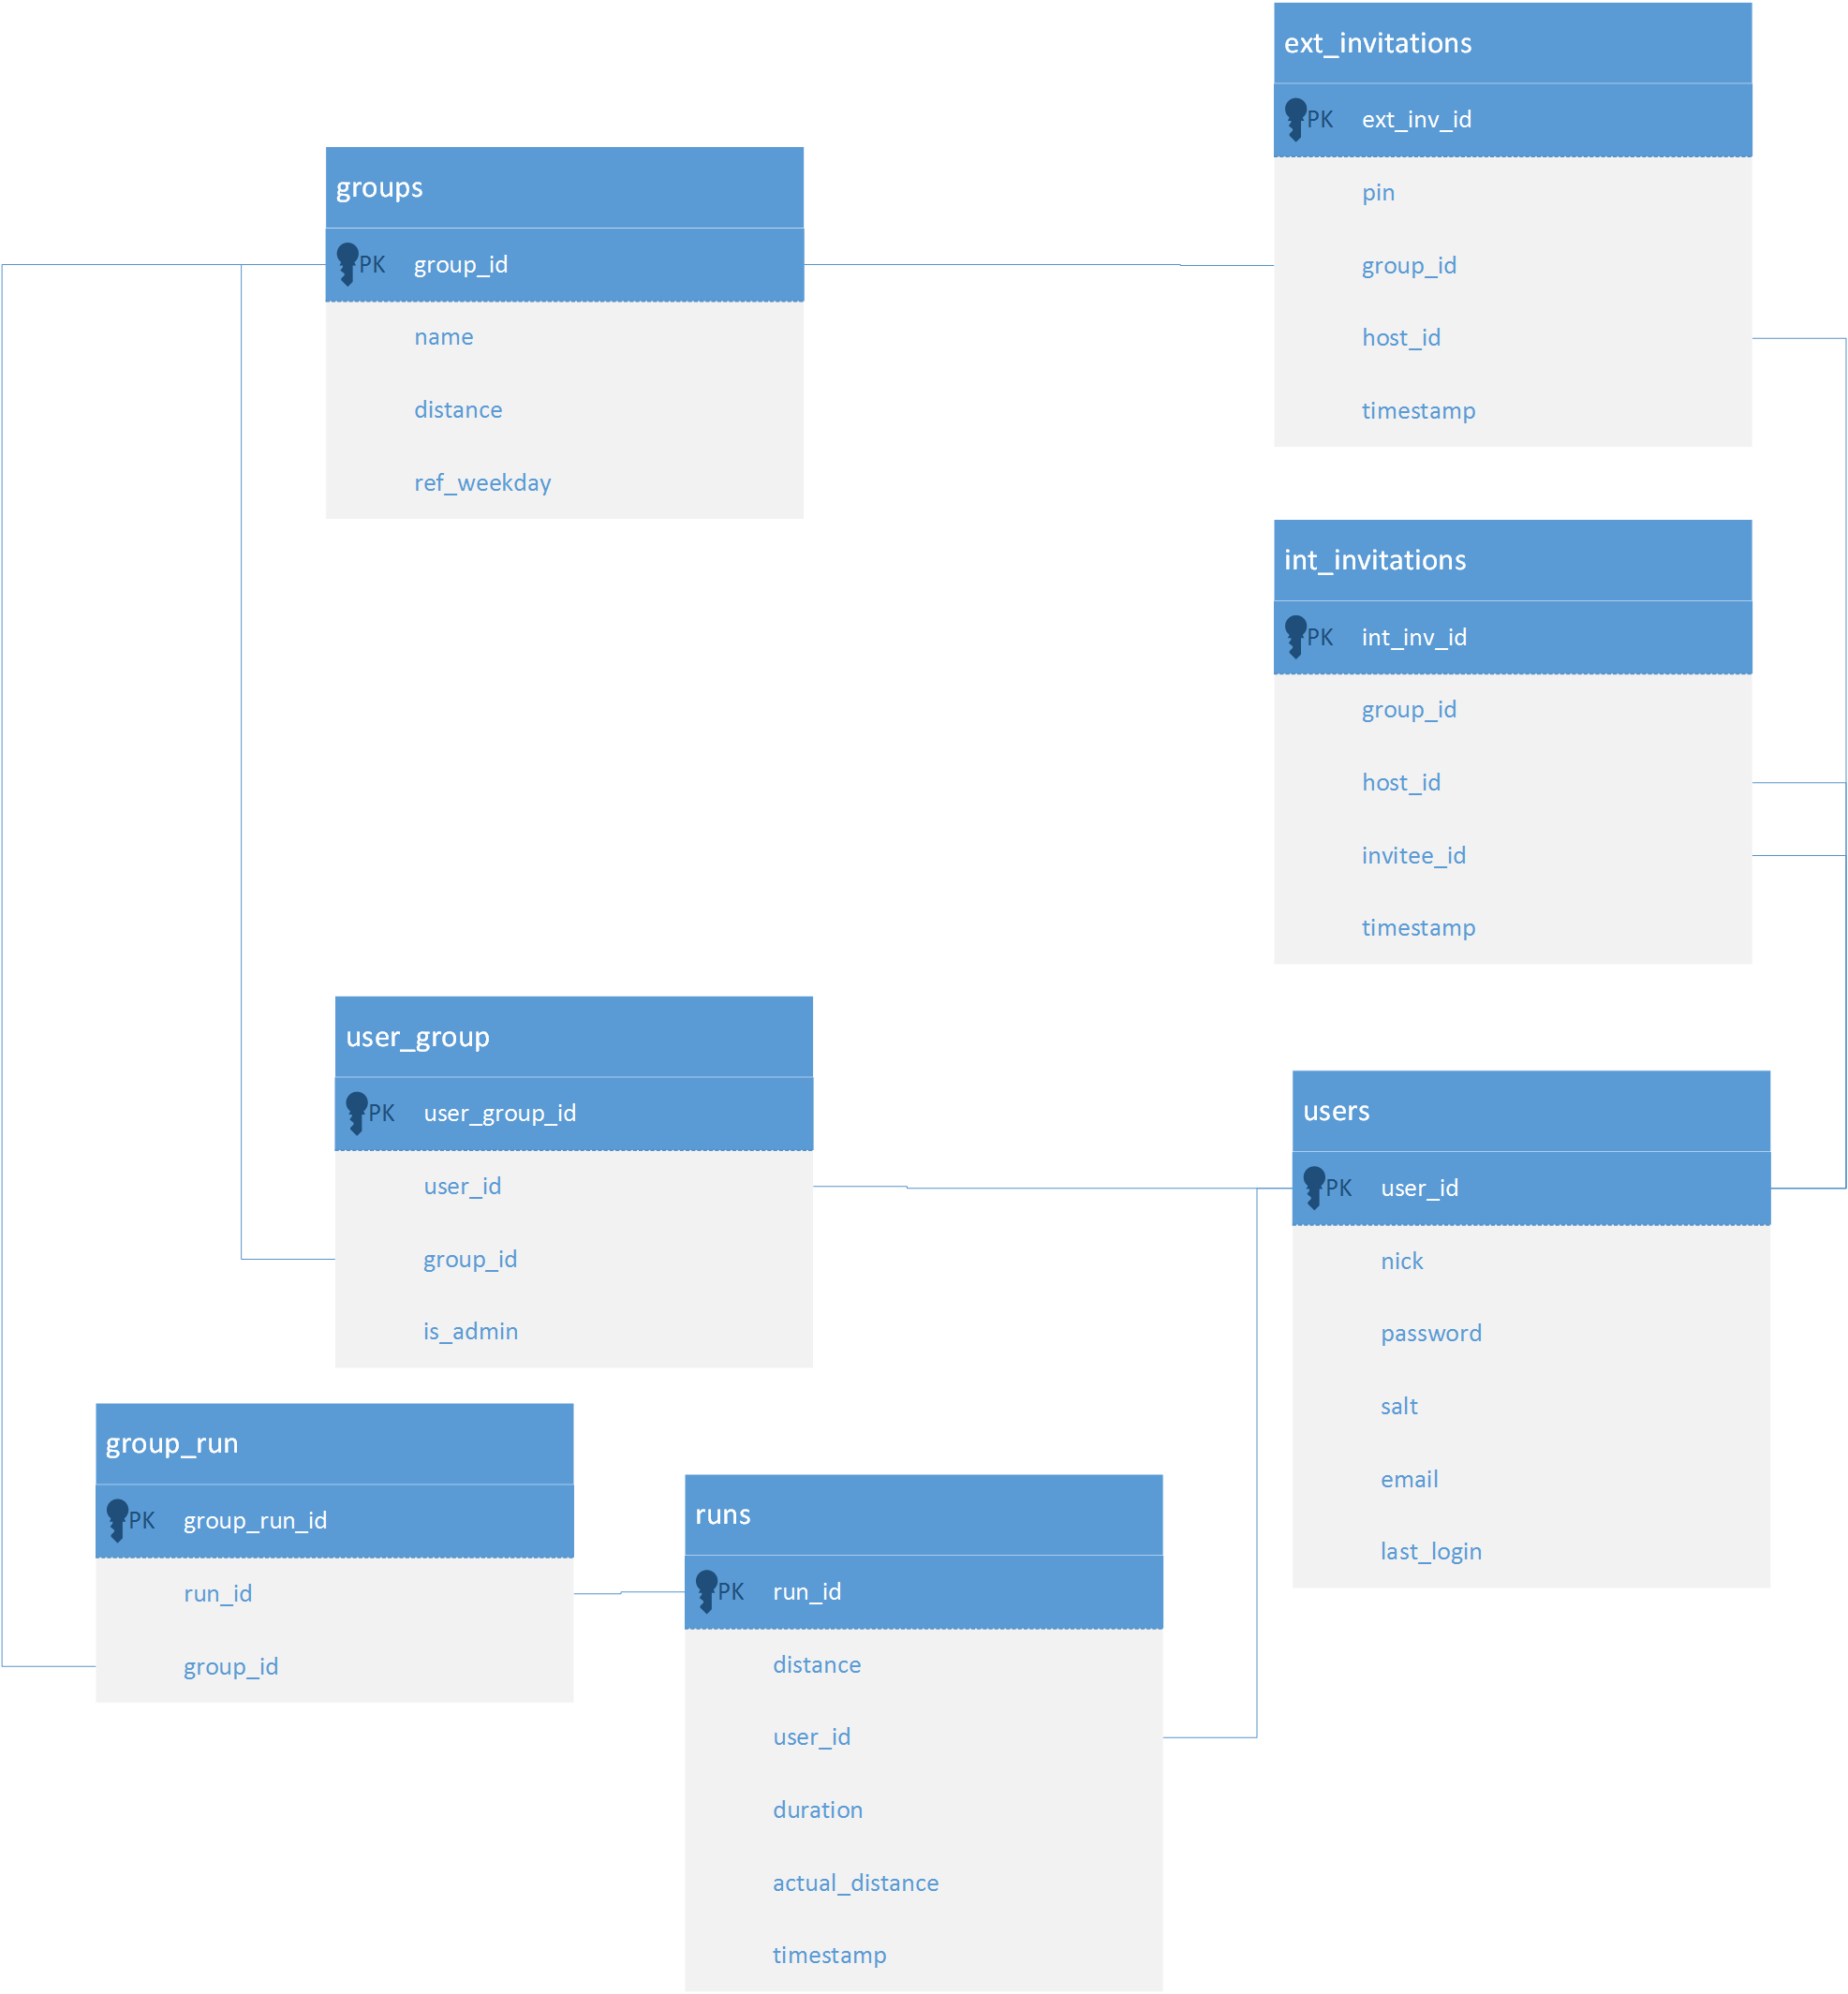
\includegraphics[width=\textwidth]{abb/er_diagram}
\caption{Datenbankschema}
\end{figure}
Die Datenbank besteht aus Tabellen für den Nutzer, die Gruppen, internen als auch externen Einladungen und den Läufen. Zusätzlich bestehen zwei weitere Tabellen für das Abbilden von n:m-Beziehungen.

Jeder Tabelle ist ein Primärschlüssel zuegordnet um eine eindeutige Identifikation jedes Tupels zu ermöglichen.

Jedem Nutzer ist ein einzigartiger Nutzername, ein verschlüsseltes Passwort, ein Salt für die Hashingfunktion, eine E-Mail-Adresse und ein Zeitstempel des letzten Logins zugeordnet.

Eine Gruppe besteht aus dem Namen, der vorgegebenen Laufdistanz und einem wöchtentlichen Stichtag, zu dem die Läufe der davorliegenden Woche ausgewertet werden. Dieser besteht aus einer Ganzkommazahl zwischen null und sechs, welche die Wochentage beginnend mit Sonntag enumeriert.

Es kann eine unbegrenzte Anzahl an Nutzern einer Gruppe beitreten und Nutzer können beliebig vielen Gruppen beitreten. Es handelt sich also um eine n:m-Relation, die anhand der Tabelle user\_group dargestellt ist. Zusätzlich wird in user\_group festgehalten, ob es sich bei dem Nutzer um einen Gruppenadministratoren handelt. Hier steht die ``1'' für ``Admin'' und die ``0'' für ``Nichtadmin''.

Eine weitere n:m-Relation mittels der Tabelle group\_run zwischen Läufen und Gruppen. Dem Lauf sind die Attribute Distanz, Nutzer-ID, Dauer, die wirkliche Distanz und ein Zeitstempel zugeordnet. Die Nutzer-ID stellt eine 1:1-Beziehung auf den Nutzer dar.

Des weiteren wurden die Tabellen ext\_invitations und int\_invitations angelegt.

Externe Einladungen sind Einladungen an Andere außerhalb der App. Es wird eine PIN geteilt, mit dem der Eingeladene später die Einladung annehmen kann. Diese ist eine 10-stellige Ganzkommazahl, Außerdem befinden sich in der Tabelle die Gruppen-ID und die Nutzer-ID, welche jeweils 1:1-Beziehungen markieren sowie ein Zeitstempel.

Interne Einladungen gehen an andere Nutzer der App. Hier sind die Attribute die ID des Einladenden, des Eingeladenen und der Gruppe. Außerdem besteht auch hier ein Zeitstempel.
%TODO Logout-->Login/Register, Kick User ist keine eigene Seite, kick nur wenn admin
\subsection{Navigationsschema}
\begin{figure}[htb]
\centering
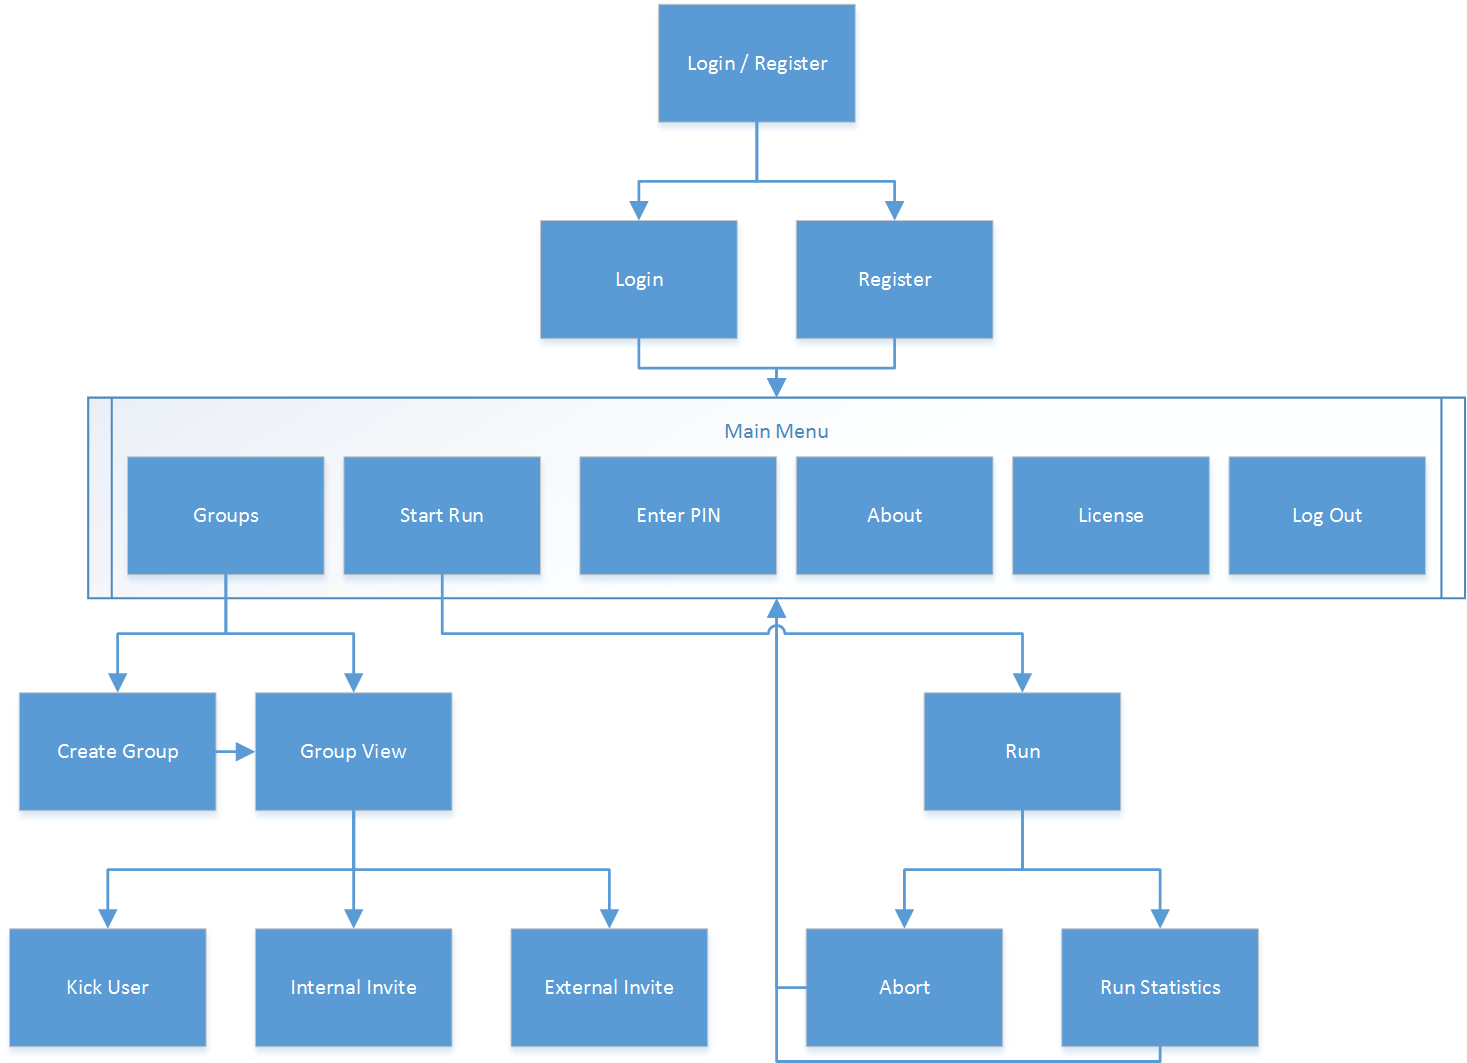
\includegraphics[width=\textwidth]{abb/navigation_diagram}
\caption{Navigationsdiagramm}
\end{figure}

%Warum was wo und wie
Nach dem Anmelden bzw. Registrieren befindet sich der Nutzer in der Gruppenübersicht. Diese ist Teil des Navigationsmenüs. Aus diesem lassen sich alle wichtigen Funktionalitäten erreichen:
\begin{itemize}
\item Gruppenübersicht - Auflistung der eigenen Gruppen und der Einladungen in Gruppen
\item Laufen - Erster Schritt zum Start des Laufs. Es wird dem Nutzer die Wahl gegeben für welche Gruppen er laufen möchte bzw. auf welcher Distanz.
\item PIN-Eingabe - Eingabe der PIN, die der Nutzer bei einer externen Einladung erhält.
\item Über - Hier stehen kurze Informationen über das Team.
\item Lizenz - Hier befindet sich die Lizenz unter der die App steht; die GNU Public License. 
\item Abmelden - Hier kann sich der Nutzer abmelden, um zurück zur Anmeldung / Registrierung zu gelangen.
\end{itemize}

Das Hauptmenü ist ein seitliches Menü, welches durch Drücken des Stapel-Icons in der oberen linken Ecke oder durch Hereinwischen vom linken Bildschirmrand erreichbar ist.

Wir haben uns für das Menü entschieden um unnötige Komplexität und Tiefe der Navigation zu vermeiden, was sowohl den Aufwand beim Programmieren der App als auch die Benutzung vereinfacht.
\subsection{Motivation}
Für viele Menschen macht Sport keinen Spaß, es ist etwas wozu sie sich zwingen müssen. Aber auch für erfahrene Athleten ist es manchmal schwierig, sich zu motivieren. Genau hier soll unsere App ansetzen, um Nutzern die Chance zu geben, sich wieder auf's Laufen zu freuen, anstatt es als Aufgabe zu sehen. Wir haben einige Punkte gesammelt, die die Motivation, zu Gh0strunner zurückzukehren erhöhen sollen.

Ein Beispiel ist die Darstellung von Geistern. Durch sie soll der läufer angespornt werden, während des Laufs sein Bestes zu geben. Am Ende des Laufs nochmal alles zu geben, um auf dem ersten Platz zu landen oder ihn zu halten, kann eine besser Motivation darstellen, als ein abstraktes "damit es einem danach besser geht".

Die Motivation soll auch zwischen den Läufen anhalten. Dafür kann der Nutzer jederzeit die vergangenen Läufe der Gruppenmitglieder ansehen und wird zusätzlich angetrieben, wenn er sieht, dass sein bester Freund gerade eine bessere Zeit gelaufen ist.

Auch funktionale Aspekte müssen für erfolgreiche Umsetzung unseres Ziels bedacht werden. Durch volle und aktive Gruppen wird der Spaß bei der Benutzung unserer App erhöht. Gruppen sollten außerdem genau einer Lauflänge zugeordnet werden, damit Nutzer stets den Überblick behalten und Gruppen wählen, in denen sie auch aktiv sind. Es macht keinen Sinn, als Anfänger einmal pro woche 20 Kilometer zu laufen. Ein sinnvoller Schritt um Gruppenbildung zu unterstützen ist es deshalb, die Anzahl der unterschiedlichen Lauflängen einzuschränken. Wir haben uns für mögliche Lauflängen von 2km, 5km, 8 km, 10km, 15km und 20km entschieden. Eine kleinschrittigere Aufteilung würde die Appnutzer auf zuviele Gruppen verteilen, wobei sie in jeder einzelnen Gruppe wahrscheinlich weniger aktiv wären.
\subsection{Laufoberfläche}
Um die Wiedererkennbarkeit und Attraktivität einer App zu haben, lohnt es sich unikate Benutzeroberflächenelemente einzusetzen. Die Stelle, an der das für unsere App sinnvoll ist, ist während dem Laufen, da alle restlichen Oberflächen hauptsächlich der Verwaltung dienen.

Wir haben uns für eine kreisförmige Darstellung der Strecke entschieden, da so einerseits der Bildschirm von Smartphones am besten ausgenutzt wird, und gleichzeitig die Assoziation zu einer Runden Strecke mit Start- und Zielline geweckt wird.

Ein farbiger Kreis soll dabei den Nutzer darstellen, der sich im Verlauf des Laufes einmal über die dargestellte Strecke bewegt. Geister werden als kleinere Kreise dargestellt, die sich mit der dauerhaft Durchschnittsgeschwindigkeit ihres Laufes bewegen. Die Abweichung zur eigentlichen Laufgeschwindigkeit zur Durchschnittsgeschwindigkeit sollte bei korrekter Wahl des Steigungsmultiplikators sowieso relativ gering sein, denn dieser soll optimalerweise die zusätzliche Anstrengung durch die Steigung ausgleichen. So kann bei der Darstellung der Geister einiges an Berechnungen eingespart werden, denn es wird nur die Zielzeit jedes Geistes benötigt.
%TODO Screenshot
Im Kreis kann der Lauffortschritt, und die aktuelle Position des Läufers gegenüber den Geistern angezeigt werden. Unter dem Kreis ist dann noch Platz für zusätzliche Laufstatistiken. 

Eine Kartendarstellung wäre ebenfalls denkbar. Wir haben uns gegen sie entschieden, da sie wo keine vorgegeben Strecke existiert sowieso nur bedingt sinnvoll wäre. Außerdem ergäbe sich durch die fehlende Möglichkeit einer ansprechenden Darstellung der Geister ein optischer Nachteil.
\subsection{Logo}
Um den Wiedererkennungswert der App zu erhöhen wurde ein Logo entworfen, welches den Inhalt wiederspiegeln sollte.

Der erste Entwurf erwies sich nach kleineren Umfragen als zu infantil.

\begin{figure}[!h]
\centering

\includegraphics[width=0.3\textwidth]{abb/icon_entwurf1}
\caption{Logo Entwurf 1}
\end{figure}
Der zweite Entwurf war etwas langweilig und zu hoch im Vergleich zu Bildbreite. 

\begin{figure}[!h]
\centering
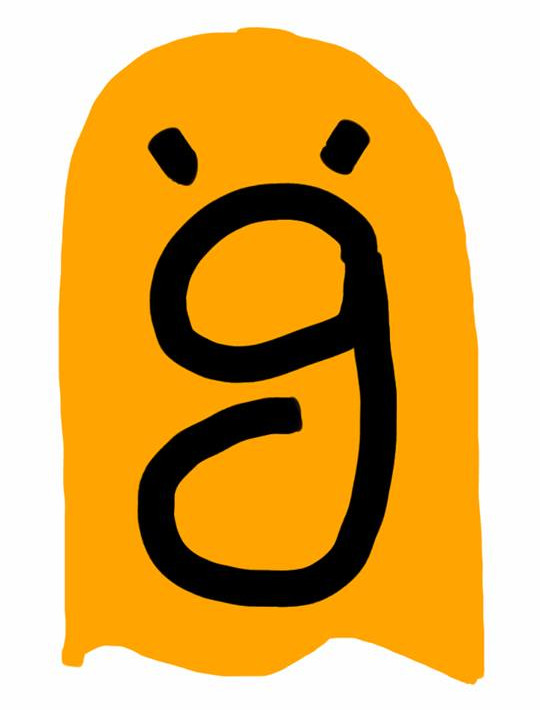
\includegraphics[width=0.3\textwidth]{abb/icon_entwurf2}
\caption{Logo Entwurf 2}
\end{figure}
Letztendlich haben wir uns für den dritten Entwurf als App-Icon entschieden, da dieses das G und R aus \textbf{G}h0st\textbf{r}unner enthält und den quadratischen Vorgaben relativ gut entspricht.
\begin{figure}[!h]
\centering

\includegraphics[width=0.3\textwidth]{abb/icon_entwurf3}
\caption{Logo Entwurf 3}
\end{figure}

%TODO Franz Tabelle URLs